\chapter{NeuroDiseases}
\label{chap:NeuroDiseases}

Another chapter dedicated to inherited neurodegenerative diseases is given in
Chap.\ref{chap:Inherited-Neurological-Diseases}. 
Magnetic resonance imaging (MRI - Chap.\ref{sec:MRI}) and positron emission
tomography (PET - Sect.\ref{sec:PET}) technologies have been critical in driving
forward our understanding of the underlying neuropathology in such disorders.

However, the relationship between underlying neuropathology and the motor,
cognitive and behavioural changes associated with many neural disorder still
remain poorly understood. As such, less conventional technologies, such as
transcranial magnetic stimulation (TMS - Chap.\ref{chap:TMS}) and
electroencephalography (EEG - Sect.\ref{sec:EEG}), provide a unique opportunity
to further investigate the causal relationships between targeted neural circuits
and objective neurophysiological responses together with overt behaviours.


Fig.\ref{fig:brain-diseases} shows brain regions affected by different
neurodegenerative diseases. Changes in gamma oscillations (20-50 Hz) have been
observed in several neurological disorders (Sect.\ref{sec:gamma-wave}). However,
the relationship between gamma oscillations and cellular pathologies is unclear.

\begin{figure}[hbt]
  \centerline{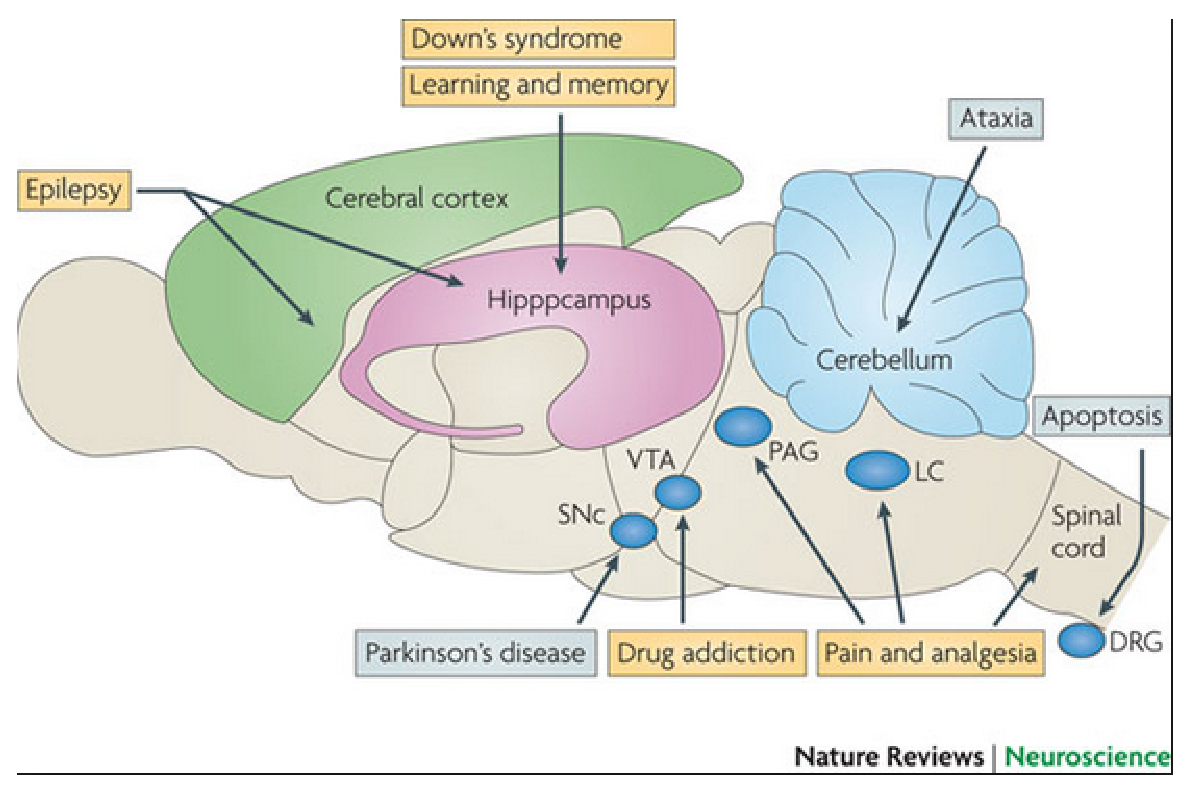
\includegraphics[height=9cm,
    angle=0]{./images/brain_diseases.eps}}
\caption{Brain Diseases
\url{http://www.nature.com/nrn/journal/v11/n5/fig_tab/nrn2834_F4.html}}
\label{fig:brain-diseases}
\end{figure}

\section{Circuit-centered view of the brain}
\label{sec:brain-disease-circuit-level}


Current understanding of neural function and dysfunction relies greatly on a
circuit-centered view of the brain.
\begin{enumerate}
  \item In Parkinson's disease:
  failure of the dopaminergic circuitry
  
  \item In Epilepsy:
  deficient inhibitory/excitatory (GABA/Glu) activity
  
  \item In memory loss:
  underperforming cholinergic activity
  
  \item In depression: 
  altered serotonergic/dopaminergic activity
  
  \item In Huntington's disease: Sect.\ref{sec:HD-theory-common-ground} 
  - not sure which circuit is causal for now though it is currently focusing
  on dysfunction in cortico-striatal projections. 
  
\end{enumerate}


\section{Diseases with effective theurapeutic developments}

Examples of pathophysiological mechanisms that have led to effective therapeutic
developments
\begin{enumerate}
  \item Parkinson's Disease (Sect.\ref{sec:Parkinson-disease}): failure in
  dopaminergic circuitry
  
  
  \item Epilepsy (Sect.\ref{sec:epilepsy_classification}): Deficient
  inhibitory/excitatory (GABA/Glu) activity
  
  \item Memory loss (Sect.\ref{sec:dementia}): underperforming cholinergic
  activity

  \item Depression (Sect.\ref{sec:depression}): altered
  serotonergic/dopaminergic activity
\end{enumerate}
\textcolor{red}{Do they links to mitochondrial dysfunction?} (at certain phases
during energy production or during mitochondrial transportation?).

\section{Alzheimer's Disease}
\label{sec:Alzheimer-Disease}


Alzheimer's disease (AD)  affects around 4 million people in the United States,
a majority of them are women who are either perimenopausal or postmenopausal
(Sect.\ref{sec:menopause-aging}). This suggests estrogen, via estrogens
receptors (Sect.\ref{sec:estrogen-receptors} the different) in the brain, may
provide a link to the disease.

AD affects several brain regions such as entorhinal cortex, hippocampus, basal
forebrain and amygdale, which exhibit synaptic loss resulting in extensive brain
atrophy.

We haven't found out exactly what starts AD process. However, we know it begins
deep in the brain. Large pyramidal neurons in the CA1 zone of hippocampus and
neurons in the basal forebrain of the {\bf entorhinal cortex} (EC)
(Sect.\ref{sec:entorhinal-cortex}) are affected in early stages of the disease.

During the pathogenesis, healthy neurons in EC begin to work less efficiently,
lose their ability to communicate, and ultimately die. The lethal process
gradually spreads to the hippocampus (Sect.\ref{sec:hippocampus}) - the brain
region that plays a major role in learning and is involved in converting
short-term memories to long-term memories.

Affected regions begin to atrophy. Ventricles, the fluid-filled spaces inside
the brain, begin to enlarge as the process continues.
{\it Scientists believe that these brain changes begin 10 to 20 years before any
clinically detectable signs or symptoms of forgetfulness appear. That's why they
are increasingly interested in the very early stages of the disease process}.
\url{https://www.nia.nih.gov/alzheimers/publication/part-2-what-happens-brain-ad/changing-brain-ad}

Alzheimer disease (AD) is considered as a multifactorial disorder involving
oxidative stress, neuroinflammation, impairments in energy metabolism, and
excitotoxicity.


\subsection{-- hypothesis}
\label{sec:Alzheimer-hypothesis}



Dr. Alois Alzheimer first described both amyloid plaques and neurofibrillary
tangles early in the twentieth century.

\begin{itemize}

  \item {\bf plaques}: (primarily made of extracellular amyloid protein, or Abeta, or Ab-42) 

The build-up of Amyloid-beta, i.e. amyloid plaques, in the extracellular
media, is found in postmortem brain

  \item {\bf neurofibrillary tangles}: (primarily made of intracellular
  phospohorylated tau protein, or hyperphosphorylated tau, or PHF-tau).
\end{itemize}

As the finding come from death patients, this information, of course, wouldn't
tell you much about when the disease started, just how it ended.


Since then, amyloid plaques and tau neurofibrillary tangles are considered as
the pathological hallmarks of Alzheimer's disease (AD). So many clinical trials
aim to reduce either or both of them, however, did not lead to any significant
improvement in clinical outcome, i.e. congitive improvement. 
A few key points
\begin{enumerate}
  
  \item  Plaques and tangles are pathological markers seen in other forms of
  dementia (and other neurological disorders as well), and not just Alzheimer's.

  \item Plaques and tangles are examples of "biomarkers" -- that is molecular
  and pathological changes that can be measured and relate to, but may or {\bf may
  not be the ultimate cause of, disease}.
  
  
  \item The exact "timecourse" of biomarkers in AD progression is still an 
  active area of research. What most scientists agree on is that  molecular
  changes may start decades before clinical symptoms are seen.
  
\end{enumerate}


\textcolor{red}{\bf Hypotheses}:
\begin{enumerate}
  \item  The build-up of peptide amyloid-beta (A$\beta$) -
  Sect.\ref{sec:amyloid-beta-Alzheimer}
  
  This build-up can be 
  \begin{enumerate}
    \item overproduction of A$\beta$
    \label{sec:Alzheimer-hypothesis-overproduction-Ab}
    
    Mutations leading to an overproduction of A$\beta$ 
    are recognized as a major cause of aggregation of the peptide in early onset familial AD

    
    \item fail to remove A$\beta$ - Sect.\ref{sec:clearance-in-brain}
    \label{sec:Alzheimer-hypothesis-impaired-clearance-Ab}
    
    Impaired clearance of A$\beta$ contributes to cerebral amyloid deposition is
    hypothesized the cause of late onset sporadic AD.
    This notion is strengthened by the finding that AD patients had identical Aβ
    production but decreased clearance rates relative to normal controls.

    
  \end{enumerate}
  
  \item tau - Sect.\ref{sec:tau-Alzheimer}
  
  \item  apolipoprotein E (APOE, Apo-E) $\varepsilon$4 allele:
   a risk factor for AD 
   
 Boxers who were APOE $\varepsilon$4 carriers were more likely to develop dementia
 pugilistica than those lacking the $\varepsilon$4 allele.
 
 ApoE isoforms exert a central role in controlling the transport of brain lipid,
 neuronal signaling, mitochondrial function, glucose metabolism, and
 neuroinflammation.
  
  \item mitochondria - Sect.\ref{sec:mitochondria-brain}
  
  \item gamma wave - Sect.\ref{sec:gamma-wave-Alzheimer}
%  \item calpain - Sect.\ref{sec:calpain-Alzheimer}

   \item GSK-3 - Sect.\ref{sec:GSK-3-in-Alzheimer}
\end{enumerate}




Other observed changes
\begin{enumerate}
  \item degeneration of cholinergic neurons in the nucleus basalis of meynert
  (Sect.\ref{sec:nucleus-basalis})
\end{enumerate}

\subsection{``Early'' biomarker detection}

Even though there is no known clinical treatment for AD, there are efforts to help early-detection.

A few assays and imaging techniquues to detect amyloid and tau in the brain and
the cerebrospinal fluid (CSF)
\begin{enumerate}
  
  \item Generally, genetic predisposition happens "first" --that is your
  genetics determine how at-risk you might be for the disease.
  
  Then, in the pre-clinical to mild stage, you may start to see changes in CSF
  tau/amyloid, followed by other markers of inflammation, oxidative stress,
  altered brain function, etc.
  
  \item   Generally, CSF Abeta changes are seen slightly earlier, while CSF tau
  changes are seen slightly later (but the exact timing varies)
  
  \item Amyloid imaging was developed in the last decade (using PIB and florbetapir), 
  
  but Tau imaging is still being developed (a number of radiotracers for imaging
  are currently under clinical evaluation.)
  
  
\end{enumerate}


\subsection{GSK-3 in Alzheimer}
\label{sec:GSK-3-in-Alzheimer}

Claudie Hooper, Richard Killick, and Simon Lovestone (2008) reviewed in ``The
GSK3 hypothesis of Alzheimer's disease''.

GSK-3 (Sect.\ref{sec:GSK3}).


\subsection{gamma reduction hypothesis}
\label{sec:gamma-wave-Alzheimer}

Iaccarino et al. (2016) showed that reduced, behaviourally driven gamma
oscillations occurs before the onset of plaque formation or cognitive decline
in a mouse model of Alzheimer's disease. Also, they showed that inducing gamma
(but not any other frequencies)  reduces levels of amyloid-$\beta$
(A$\beta$)1-40 and A$\beta$ 1-42 isoforms in the visual cortex of of
pre-depositing mice and mitigated plaque load in aged, depositing mice.

\begin{mdframed}

Gamma wave was induced using optogenetically driving fast-spiking
parvalbumin-positive (FS-PV)-interneurons at gamma (40 Hz).

\end{mdframed}


The question is
\begin{enumerate}
  \item  Gamma does what to the formation of plaque ????
  
  \item 
\end{enumerate}




\subsection{tau hypothesis}
\label{sec:tau-Alzheimer}

When a brain affected by Alzheimer's disease is examined, all six isoforms of
tau (Sect.\ref{sec:tau-protein}) are often found hyperphosphorylated in paired
helical filaments.

Tau hypothesis (however, tauopathies is not unique to AD; it is also found in
about 20 other neurodenegerative disorders - Sergeant et al., 2005)
\begin{enumerate}
  \item lead to elevated calpain-1 activity (Sect.\ref{sec:calpain-1})
  
  \item 
\end{enumerate}

Analysis of human brain has shown that calpain activity is elevated in AD
compared to controls, and that calpain-mediated proteolysis regulates the
activity of important disease-associated proteins including the tau kinases
cyclin-dependent kinase 5 and glycogen kinase synthase-3

Increases in calpain-1 activity were associated with elevated activity of the
endogenous calpain inhibitor, calpastatin, itself a known calpain substrate.
Activation of the tau kinases, glycogen-kinase synthase-3 and cyclin-dependent
kinase 5 (CDK5 - Sect.\ref{sec:CDK5}) were also found to occur in Braak stage
II-III brain, and these preceded global elevations in tau phosphorylation and
the loss of post-synaptic markers.



\subsection{amyloid-beta hypothesis}
\label{sec:amyloid-beta-Alzheimer}

It is observed that amyloid-beta build up in AD patients
(Sect.\ref{sec:Alzheimer-Disease}). However, pharmacological efforts to reduce
the buildup have not showed the effective.
There are two amyloid-beta: A$\beta$-40 and A$\beta$-42. However,
A$\beta$-42 aggregation, and not A$\beta$-40, is the marker that is close to
Alzheimer aetiology. (Sergeant et al., 2005).

It has been believed that only neurons produced toxic A$\beta$.
However, recent evidences suggested that  associated astrocyte can make
and secrete increased amounts of endogenous A$\beta$-42 (Dal Pra et al., 2015).

It is hypothesized that the aggregation of this peptide somehow causes
dysregulation of synaptic plasticity and eventually causes destruction of
synapses and neurons. Proposed mechanisms by which excessive level of A$\beta$
(Sect.\ref{sec:amyloid-beta}) mediates its effects include
\begin{enumerate}
  \item lipid destabilization, 
  
  \item activation of native membrane channels, and
  
  \item aggregation of A$\beta$ into Ca2+-permeable pores.
\end{enumerate}

\subsection{-- forming Ca2+-permeable pore}

In 1992, Hardy and Higgins reported findings that suggested a new and intriguing
possibility; in that A$\beta$ peptides disrupt Ca2+ homeostasis in neurons and
increase intracellular Ca2+ [Ca2+]i.
\begin{itemize}
  \item  A$\beta$ exposure to human cortical neurons raised [Ca2+]i (Mattson, Cheng et
  al 1992); (Hardy and Higgins 1992).
  
  \item A$\beta$ peptides might function like Ca2+ ion channels (Arispe et al 1993). 
\end{itemize}


\section{Cortical spreading depression (CSD)}
\label{sec:cortical-spreading-depression}

In the evolution of the cerebral cortex, the sophisticated organization in a
steady state far away from thermodynamic equilibrium has produced the side
effect of two fundamental pathological network events: ictal epileptic activity
(Sect.\ref{sec:epileptic-seizures}) and spreading depolarization.

\begin{mdframed}

Spreading depolarizations (SD) are waves of abrupt, sustained (i.e.
near-complete breakdown) of neuronal transmembrane ion gradients, are the
largest possible pathophysiologic disruption of viable cerebral gray matter.

The wave propagate at velocities of 1.7-9.2 mm/min in
gray matter of the brain.

It originates in neurons and is characterized by active propagation of an
abrupt, near-complete breakdown of the neuronal transmembrane ion gradients, in
contrast to the slow breakdown that can be observed in any cell of the body
before death when there is severe energy deprivation.
\url{https://www.youtube.com/watch?v=UkT65Y4iFrk}

The concentration gradient of practically {\it every investigated small molecule
changes} between cytoplasm and interstitial space during SD.
In addition, cell organelles such as mitochondria undergo marked alterations
during SD.

\end{mdframed}

CSD was discovered in 1944 by Leo; yet we still do not have a detailed
understanding of how CSD is manifest.  Recently, unequivocal
electrophysiological evidence has been found in patients that spreading
depolarizations occur abundantly in stroke and brain trauma.

CSD has been associated with massive changes in cortical perfusion.
Blood delivery is known to play a significant role in CSD in several ways.
Focal ischemia causes spreading depolarization within minutes
(Sect.\ref{sec:CSD-role-of-ischema}).

\begin{mdframed}

Experiments to induce SD: SD can be detected via 
\begin{enumerate}

  \item  the abrupt extracellular concentration changes of glutamate, potassium,
  or sodium using microelectrodes in vivo or in brain slices

  \item the large increase in intracellular calcium as measured with calcium
  imaging

  \item the cellular swelling and dendritic beading as observed with
two-photon microscopy, which is associated with
shrinkage of the extracellular space

  \item the local
decrease in intracellular water mobility as imaged by
diffusion-weighted magnetic resonance imaging
(MRI)

  \item the release of free energy from the tissue that is converted to heat
  (''free energy starving'')

  \item  SD involves astrocytes, provokes marked microvascular/hemodynamic
responses, activates microglial cells and
inflammasome formation and induces cytokine gene
expression.

\end{enumerate}

SD creates an interface of reciprocal interaction between the three super
systems -  nervous, vascular, and immune - whenever the brain is locally injured.
This interface reaches far beyond the actual zones of injury because of the
spreading nature of SD. It is suggested that this phenomenon is among the most
fundamental processes of brain pathology.

SD monitoring can be performed at the bedside, continuously, and in real time.
\end{mdframed}

As a rule of thumb, changes during SD are at least five times greater than those
observed during IEE (Sect.\ref{sec:epileptic-seizure}).

\begin{enumerate}
  \item  common to all species tested is a mismatch in the delivery of
  substrates to meet metabolic demands, resulting in a derangement of
  neurovascular coupling 
  
  \item Changes in perfusion can induce peri-infarct depolarizations (PID),
  which are electrophysiologically identical to CSD.
  
Conditions that mimic the effects of hypoperfusion, such as oxygen glucose
deprivation (OGD) and exposure to ouabain (an inhibitor of the Na/K-ATPase),
also generate spreading depolarizations 

  \item Perfusion changes can also modulate the signature characteristics of
  CSD. Depending on the levels of the underlying oxygenation or blood pressure,
  the amplitude and duration of depolarization and the velocity of propagation
  of CSD can be altered  

\end{enumerate}

A principal role of astrocytes is the clearance of local increases of ECS
potassium. Previous mathematical models of CSD have accounted for ionic
diffusion [16], cellular membrane ionic currents [16], [17], the -ATPase and
other membrane pumps [16], [17], and extra- and intracellular volume changes
[18][20].
\begin{enumerate}
  \item Chang et al. (2013): incorporate astrocyte effects through empirical
  potassium buffering.
  
as they are not interested in the exact mechanisms of glial potassium buffering,
but are interested in reproducing accurate potassium dynamics for our model
  
  \item 
\end{enumerate}

\subsection{CSD: role of ischema}
\label{sec:CSD-role-of-ischema}

Focal ischemia causes spreading depolarization within minutes The incidence of
ischaemia in patients with severe TBI detected with radio active
$^{133}$Xe as tracer, using xenon CT is high (30-45\% of patients).
A recent study detected a much higher (79\%) incidence of ischaemia detected,
which was likely attributable to the use of continuous, rather than
intermittent, perfusion monitoring.

Spreading depolarizations exacerbate neuronal injury through
prolonged ionic breakdown and spreading depolarization-related hypoperfusion
(spreading ischemia). Local duration of
the depolarization indicates local tissue energy status and risk of injury.

Focal cerebral ischaemia experiments have suggested cerebral blood flow 518
ml/100 g/min as an infarction threshold, which if maintained over some hours,
causes irreversible tissue damage (Jones et al., 1981). This ischaemic threshold
has been widely adopted in experimental and clinical studies, regardless of the
techniques used.

\begin{itemize}
  \item  increased perfusion is associated with better outcomes
(Obrist et al., 1984; Marion and Bouma, 1991; Marion
et al., 1991; Bouma et al., 1992; Muizelaar and Schroder, 1994;
Schroder et al., 1996; hinzman, 2014)


\end{itemize}


\section{Tourette's Syndrome}
\label{sec:Tourette-syndrome}


Tourette's syndrome is one type of {\bf Tic Disorder} and is linked to childhood
onset (can last for years or even lifelong). The other types are {\it Chronic
Tic Disorder} (Motor or Vocal Type), and {\it Provisional Tic Disorder}.
The habitual spasmodic contraction of the muscles, most often in the face, or
diosyncratic and habitual feature of a person's behavior is called {\bf tics}.
Tics are involuntary, repetitive movements and vocalizations.
The three Tic Disorders are distinguished by the types of tics present (motor,
vocal/ phonic, or both) and by the length of time that the tics have been
present.

Patients with  Tourette's syndrome  have at least two motor tics (such as
repeatedly blinking the eyes, shrugging shoulders) and at least one vocal/
phonic tic in some combination (unwanted sounds, or blurting out offensive
words) over the course of more than a year.
According   to DSM-IV-TR (American   Psychiatric Association, 2000), it is
characterized by brief, stereo- typical, but {\it nonrhythmic} movements and
vocalizations called tics. Common tics include eye blinking, grimacing, jaw,
neck, shoulder or limb movements, sniffing, grunting,  chirping,  or  throat 
clearing.
\begin{itemize}
  \item motor tics often begin between the ages
of 3 and 8, several years before the appearance of vocal
tics

  \item Only   20\%   or   fewer   of   children   with   TS
continue to experience a moderate level of impairment
of global functioning by the age of 20 years (Bloch et al., 2006a).

  \item Tic  disorders   that  persist  into
adulthood  can  be  associated  with  the  most  severe symptoms  including 
violent  episodes  of  self-injurious motor tics  (secondary  to  hitting or
biting)  or socially stigmatizing  coprolalic  utterances  or  gestures  (e.g.,
shouting obscenities or racial slurs)

Tics   are   also   sensitive   to   a   number   of   factors
including  everyday  psychosocial  stress,  anxiety,  emo-
tional  excitement,  and  fatigue  (Findley  et  al.,  2003;
Hoekstra  et  al.,  2004a).   
Interestingly,  activities  that require focused attention and fine motor
control, such as   reading   aloud,   playing   a   musical   instrument,
engaging   in   certain   sports   (and   even   performing surgery)  are 
commonly  associated  with  the  transient disappearance of tics

Although  much  diminished,  tics  can  occur  during
sleep (Sect.\ref{sec:sleep}). 
 
  \item Tics often occur in discrete {\bf bouts} over time scales of
days to years (Peterson and Leckman, 1998)

Bouts (i.e. short period of intense activity of a specified kind)
is characterized by brief  periods  of  stable  intertic
intervals of short duration, typically 0.5 to 1.0 seconds.

A deeper understanding of these events may occur  as  we  begin  to  understand 
the  neural  events involved in tic generation (at the millisecond time scale)
(Leckman et al., 2006).



\end{itemize}

\begin{mdframed}

Individuals with Chronic Tic Disorder have either motor tics or
vocal tics that have been present for more than a year, and individuals with
Provisional Tic Disorder have tics that have been present for less than a year.

\end{mdframed}

he pattern of hereditary transmission, in which twin studies revealed high
concordance rates in   monozygotic   but   not   dizygotic   twins,   initially
suggested  major  gene  effect.
Early studies suggested the  importance of   several   chromosomal   regions,
including   11q23 (Merette et al., 2000), 4q, and 8p. However, recent finding
suggested vulnerability genes in different regions. They implicate regions near
the {\it centromere of chromosome 2 as well as 6p, 8q, 11q, 14 q, 20q, 21q}
(Simonic et al., 1998),  and {\it chromosome X}  (Diaz-Anzaldua  et  al., 2004).
\begin{enumerate}
  \item 
  X-linked vulnerability gene was ruled out; and the linked to male
  was hypothesized by the presence of androgenic steroid during critical periods
  in fetal development  (Peterson
et al., 1998b, Alexander  and
Peterson, 2004).

  \item Temperature dependent causing the change in hypothalamic function: This
  increase in tics was   correlated   with   their   local   sweat   rate   via 
   a dopamine-mediated pathway in the hypothalamus.
  
  \item  Verkerk et al. (2003) reported the
  disruption of the {\bf contactin-associated protein 2} gene on chromosome 7. This gene
encodes a membrane protein located  at  nodes  of  Ranvier  of  axon that may be important
for the distribution of the K+ channels, i.e. affect signal conduction along
myelinated neurons.

  \item  Mutations in SLITRK1 gene on chromosome 13q31.1 is considered as a
  rare cause (1-2\% in patients) of Tourette's sydnrome (Abelson et al. (2005)).
\end{enumerate}

With rare exceptions, such as SLITRK1 , it is likely that  multiple 
vulnerability  genes  involve in the disease.


\url{http://neurowiki2014.wikidot.com/individual:individual-subtopic}


\section{Parkinsonism}
\label{sec:Parkinsonism}

Syndromes considered as Parkinsonism: (1) bradykinesia, (2) hypokinesia, (3)
cogwheel rigidity, (4) postural instability, (5) resting tremor.
They are found in patients with significant decrease in domapine in CNS
(Sect.\ref{sec:dopaminegic_pathways}).

Reduction in dopamine can be caused by different factors (unknown which one is
major to PD)
\begin{enumerate}
  \item  intoxication (substance abuse)
  \item   traumata
  \item   vascular alterations
  \item   infections
  \item   genetically based familial forms of Parkinsonism
  \item   degenerative disease (tauopathies progressive suprenuclear palsy (PSP), Alzheimer's disease)
  \item   synycleinopathies multiple system atrophy (MSA)

  \item   Lewy body disease (LBD - Sect.\ref{sec:lewy-body-disease} - 3 related
  subentities: pure autonomic failure (PAF), sporadic (idiopathic) Parkinson
  disease (PD), and diffuse Lowey body disease (DLBD)

**Sporadic Parkinson disease is the most common form of parkinsonism
 
\end{enumerate}
{\small
\begin{verbatim}
---> pathological process linked to the formation of aberrant proteinaceous inclusion bodies 
      in a limited # of neural types distributed throughout PNS/ENS/CNS
      (peripheral/enteric/central)

---> but do not routinely accompany aging
\end{verbatim}
}

\section{Lewy Body Disease (LBD)}
\label{sec:lewy-body-disease} 

In the early 1900s, while researching Parkinson's disease, the scientist
Friederich H. Lewy discovered abnormal protein deposits that disrupt the brain's
normal functioning.

{\bf Lewy bodies} are abnormal aggregates of protein called alpha-synuclein that
develop inside the bodies of nerve cells (Sect.\ref{sec:alpha-synuclein}). 

Lewy bodies are found in an area of the brain stem where release of the
neurotransmitter dopamine are low or depleted, causing Parkinsonian symptom;
then these abnormal proteins are diffuse throughout other areas of the brain,
including the cerebral cortex.

Eventually, the brain chemical acetylcholine is depleted, causing disruption of
perception, thinking and behavior. Lewy body dementia exists either in pure
form, or in conjunction with other brain changes, including those typically seen
in Alzheimer's disease and Parkinson's disease.

Nowadays, Lewy Body Disease (LBD) is an umbrella term refering to dementia, i.e.
memory loss, that worsen over time that can be in one of 3 related subentities
\begin{enumerate}
  
  \item pure autonomic failure (PAF), 
  
  \item sporadic (idiopathic) Parkinson disease (PD), and  
  
  \item diffuse Lewy body disease (DLBD)
  
\end{enumerate}

LBD is NOT a rare disease, and affects an estimated 1.4 million individuals
and their families in the United States.


% \subsection{alpha-synuclein}
% 
% Sect.\ref{sec:alpha-synuclein}.
  
  
\section{-- (Sporadic) Parkinson disease}
\label{sec:Parkinson-disease}


Sporadic (idiopathic) Parkinson disease is the most common form of parkinsonism
(Sect.\ref{sec:Parkinsonism}) with the characteristic bradykinesia (slowness),
rigidity and tremor of PD which are primarily due to an underlying degeneration
of dopaminergic nigrostriatal neurons and the resultant depletion of striatal
dopamine.


The most prominent pathological change in idiopathic parkinsonism is
degeneration of the {\it nigrostriatal dopaminergic pathway}
(Sect.\ref{sec:nigrostriatal-pathway}) with nerve cell loss in the substantia
nigra pars compacta (SNpc - Sect.\ref{sec:SNpc}).


The cause of death of dopaminergic neurons in the pars compacta is unknown.
However, Parkinsonian symptoms do not appear until up to 50-80\% of pars
compacta dopaminergic neurons have died.

Different hypotheses:
\begin{itemize}
  
  \item abnormalities in mitochondrial Complex 1
  (Sect.\ref{sec:complex-I-mito}), causing aggregation of alpha-synuclein
  (Sect.\ref{sec:alpha-synuclein}); this can result in abnormal protein handling
  and neuron death
  
  \item less calbindin (fast $\Ca$ binding proteins - Sect.\ref{sec:calbindin})
  than other dopaminergic neuron, i.e.  increasing free $\Ca$ level and thus
  leading to toxicity. Here, it is hypothesized that metabolic stress created by
  sustained Ca2+ entry, i.e.
   the engagement of L-type Ca2+ channels during autonomous pacemaking elevates
  the sensitivity of SNc DA neurons to mitochondrial toxins.
    
  Surmeier et al. showed that it is L-type $\Ca$ channel that drive
  spontaneous activity of A9-DA neurons (A9 group dopamine neuron in SNpc) - a
  key component of their selective vulnerability. 
  
  
  \item NMPTP (a neurotoxic agent) can induce similar neurological disorder in
  Parkinson disease (i.e. drug-induced Parkinsonism) - Sect.\ref{sec:NMPTP}.
  
  However, it causes only damaging the neurons in substantia nigra pars compacta
  (corresponding to A8 and A9 cells in the rat brain), but no damage found
  dopamine terminals in the nucleus accumbens and olfactory tubercule projected by
  dopaminergic neurons in the ventral midbrain (corresponding to A10 cells in
  the rat brain).
  It suggested these two dopaminergic neuronal systems are different in
  sensitive to neurotoxin \citep{burns1983}.
  
   
  \item exaggerated beta oscillation (15-30Hz) within cortico-basal
  ganglia-thalamic (CBT) neural network - Sect.\ref{sec:beta-wave}
  
\end{itemize}

\subsection{NMPTP}
\label{sec:NMPTP}

MPTP (1-methyl-4-phenyl-1,2,3,6-tetrahydropyridine) 
is not directly harmful, yet in the brain, MPTP can be metabolized into
the toxic cation 1-methyl-4-phenylpyridinium (MPP+) by the enzyme MAO-B of glial
cells (Sect.\ref{sec:glial-cells}). MAOB (Monoamine oxidase B) is an enzyme
located in the outer mitochondrial membrane.
 
So, MPTP is a neurotoxin precursor to MPP+ (Sect.\ref{sec:MPP+}), which causes
permanent symptoms of Parkinson's disease by destroying doparminergic neurons in
SNpc \citep{burns1983}. Injection of MPTP causes rapid onset of
Parkinsonism.
MPTP can be accidentally produced during the manufacturing of MPPP.
The Parkinson-inducing effects of MPTP were first discovered following
accidental ingestion as a result of MPPP contaminated with MPTP.

NMPTP is N-methyl-4-phenyl-1,2,3,6-tetrahydropyridine.
In animal injected with NMPTP, tissues were analyzed for homovanillic acid
(HVA), 5-hydroxyindoleacetic acid (5-HIAA), 3-methoxy-4-hydroxyphenylethylene glycol
(MHPG) and dopamine. The concentration of all of them have been reduced in
ventricular cerebrospinal fluid (CSF) \footnote{homovanillic acid (HVA) is the
major  metabolite of dopamine;  5-hydroxyindoleacetic acid (5-HIAA) is the main
metabolite of serotonin  (Sect.\ref{sec:serotonin}); 3-methoxy-4-hy-
droxyphenylethylene glycol (MHPG) is a metabolite of norepinephrine
degradation}.

\subsection{MPP+}
\label{sec:MPP+}

MPP+ (1-methyl-4-phenylpyridinium) is a positively charged molecule with
chemical formula \ce{C12H12N+}
which can be generated from MPTP (Sect.\ref{sec:NMPTP}).

MPP+ cause neuronal death selectively to dopaminergic cells
(Sect.\ref{sec:dopaminegic_neurons}) via the DA transporter
(Sect.\ref{sec:DA-transporter}) - a mechanism that help reuptaking DA back into
the cells after DA release \citep{gainetdinov1997}.
 
It is suggested that MPP(+) neurotoxicity is a multi-component process involving
both
\begin{enumerate}
  \item mitochondrial dysfunction: MPP+ inhibit complex I of mitochondria
  (Sect.\ref{sec:complex-I-mito}), i.e. leading to the depletion of ATP and causing cell death.

  
  \item ROS generated by vesicular DA displacement: 
  inhibits the synthesis of
  catecholamines, reduces levels of dopamine and cardiac norepinephrine, and inactivates tyrosine hydroxylase
  
  MPP(+)-induced ROS formation is not mitochondrial in origin but results from
  intracellular dopamine (DA) oxidation.
\end{enumerate}

Although intracellular iron plays a crucial role in MPP(+)-induced apoptosis,
the molecular signalling mechanisms linking iron, reactive oxygen species (ROS)
and apoptosis are still unknown - Sect.\ref{sec:apoptosis}.

  
\subsection{Drugs}
\label{sec:Parkinson-drug-therapy}

Despite several available therapeutic options to treat the symptoms of
Parkinson's disease (PD), there are currently no agents that halt or slow the
progression of disease.

Repleting endogenous dopamine using its precursor L-dopa and mimicking it using
dopamine agonists constitute 'dopamine replacement' strategies - the mainstay of
current treatment; yet none of that currently alter the underlying degeneration
of dopaminergic neuron. So, such treatments can only be useful when the neuron
loss is not worse. Thus, after several years of gratifying improvement using
dopamine-replacement therapy, PD patients typically experience great frustration
as neuronal loss and symptoms inexorably progress.

{\bf levodopa}, a precursor for the neurotransmitter dopamine, currently the
drug-of-choice in treatment of Parkinson's disease. Drug trade names supplying
levodopa: Sinemet, Pharmacopa, Atamet, Stalevo, Madopar, and Prolopa.
There is also the risk of predominant l-DOPA-related onset of motor
complications in addition to its direct ameliorating effect on motor symptoms
Dopamine-substituting drugs may dose-dependently produce systemic side effects,
particularly onset of hypotension and nausea by peripheral dopamine receptor
stimulation. 
 
{\bf nobiletin} - a flavonoid found in citrus - can rescue dopaminergic neurons
from degeneration caused by MPP+. Nobiletin was shown to augment AMPA receptor
activity and long-term potentiation in cell culture.


As activation of A2A receptors co-localize with D2-receptors and oppose the
activation of D2R. Antagonism of the A2A receptor improves motor behavior in
patients with Parkinson's disease (PD). {\bf Antagonists of adenosine A2A
receptors} have recently emerged as a leading candidate class of non-
dopaminergic anti-parkinsonian agents
(Sect.\ref{sec:A2A-receptor-D2-receptor-heteromer}).
\begin{enumerate}
  \item  {\bf istradefylline} - a xanthine derivative, is a selective A2A
  receptor antagonist with longest half-life out of the available A2A receptor
  antagonists.  Istradefylline easily crosses the blood-brain barrier and shows
  a high affinity to the human A2A receptor.
  
  Istradefylline has shown (modest) efficacy in phase II trials (Hauser
  et al., 2003), which were considered promising enough to justify phase III
  clinical trials (Schapira et al., 2006).
  Istradefylline reduces dyskinesia resulting from long-term treatment with
  classical antiparkinson drugs such as levodopa. Istradefylline is an analog
  of caffeine. 
  
   
   At 2012, istradefylline is not yet an FDA-approved drug (Park, Stacy 2012).
   %https://www.ncbi.nlm.nih.gov/pubmed/22149371
   
   
  \item related selective antagonists are also being tested (Schapira et al., 2006).    
\end{enumerate}


\subsection{Genes in PD}

Early evidences starting in 1996 suggested the first mutation responsible for
PD.  In 1998, two chromosomal regions were reported. In 2012, there are 28
distinct chromosomal regions more or less convincingly related to PD. It then became
clear that PD is a genetically heterogeneous and most likely, complex disorder.

 
\subsection{Monogenics form of Parkinson Disease (PD)}

Monogenic forms, caused by a single mutation in a dominantly or recessively
inherited gene are well-established, albeit relatively rate in PD.
There are 6 chromosomal regions contain genes with mutations that conclusively
cause monogenic PD; yet they collectively account for about 30\% of the familial
and 3\%-5\% of the sporadic cases.


PARK is the term referring to 18 specific chromosomal regions, also called
chromosomal locus, and are numbered in chronological order of their
identification (PARK1, PARK2, PARK3, \ldots) - (Klein, Westenberger, 2006). 
\begin{itemize}
  \item PARK1 (chromosome: 4q21-22): gene SNCA (Sect.\ref{sec:SNCA-gene}) -
  disorder EOPD
  
  \item PARK2 (6q25.2-q27)
  \item PARK3 (2p13): classical PD
  \item PARK4 = PARK1
  
  \item PARK5 (4p13): gene UCHL1
  \item PARK6 (1p35-p36): gene PINK1
  \item PARK7 (1p36): gene DJ-1
  \item PARK8 (12q12): gene LRRK2
  
{\it LRRK2} is a large gene that consists of 51 exon, encoding 2527-amino acid
cytoplasmic protein leucine-rich repeat kinase 2 (LRRK2). It is the most
frequent known cause of late-onset autosomal-dominant and sporadic PD, with a
mutation frequency ranging from 2\% to 40\% in different populations.
At least 16 out of more than 50 different missense and non-sense mutations
(including the six recurrent mutations-p.R114C, p.R1441G, p.R1441H, p.Y1699C,
p.G2019S, and p.I2020T) seem to be pathogenic.

  \item PARK9 (1p36): gene ATP13A2
  \item PARK10 (1p32): 
  \item PARK11 (2q36-27): late-onset PD
  
  \item \ldots
\end{itemize}
\url{http://www.ncbi.nlm.nih.gov/pmc/articles/PMC3253033/table/A008888TB1/}



\section{Menopause and Aging: Neuro function}
\label{sec:menopause-aging}

A menopause = a decline in reproductive hormone, which typically happens to
woman at the age of 40s or 50s. This reproduction may causes several changes to
the body, including nerve symptoms.

{\bf Surgical menopause} = A menopause caused by unusual event, e.g. when the
overies are surgically removed (e.g. by bilateral oophorectomy or the ovaries
are greatly damaged by radiation, chemotherapy or other medications).
This causes an abrupt menopause, with women often experiencing more severe
menopausal symptoms than they would if they were to experience menopause
naturally.

{\bf Hormone (replacement) therapy} (HRT, e.g. estrogen replacement) was once
routinely used to treat menopausal symptoms and protect long-term health.
\textcolor{red}{Then large clinical trials showed health risks, particularly
when given to older postmenopausal women}. Hormone therapy is no longer
recommended for disease prevention, such as heart disease or memory loss.


It has been suspected that  estrogen deficiency at menopause might modulate the
course of age-related cognitive decline, especially short-term memory in the
hippocampus \citep{rapp2003} (Sect.\ref{sec:hippocampus}). The
hormone-replacement regimen can also induces spine proliferation in monkeys, in both the hippocampus and prefrontal cortex
\citep{hao2007}.


\section{Major Depression Disorder (MDD): major
depression, recurrent depressive disorder, clinical depression,
unipolar depression, or unipolar disorder}
\label{sec:MDD}
\label{sec:unipolar-disorder}


Depression is a common disorder, affecting over 120 million people worldwide, 
with  lifetime prevalence of depression is in the range of 10\% to 15\%
(Lepine, Briley, 2011; Nikolaus et al., 2012)
\begin{itemize}
  \item 
\end{itemize}

\section{Psychosis}
\label{sec:psychosis}

Psychosis is an abnormal condition of the mind that involves a "loss of contact
with reality". The term "psychosis" is very broad and can mean anything from
relatively normal aberrant experiences through to the complex and catatonic
expressions of schizophrenia (Sect.\ref{sec:schizophrenia}) and bipolar type 1
disorder (Sect.\ref{sec:bipolar-type-1}).

NOTE: Amphetamine can also induced psychoses (Sect.\ref{sec:amphetamine}).

\section{-- Bipolar disorder: type-1 and type-2}
\label{sec:bipolar-disorder}

\subsection{Bipolar type-1}
\label{sec:bipolar-type-1}

Bipolar I disorder (BP-I; pronounced "type one bipolar disorder") is a bipolar
spectrum disorder (Sect.\ref{sec:bipolar-disorder}) characterized by the
occurrence of at least one manic or mixed episode.

The essential feature of bipolar I disorder is a clinical course characterized
by the occurrence of one or more manic episodes or mixed episodes (DSM-IV-TR,
2000). One episode of mania is sufficient to make the diagnosis of bipolar
disorder.

\url{https://en.wikipedia.org/wiki/Bipolar_I_disorder}


\subsection{Bipolar type-2}
\label{sec:bipolar-type-2}

Unlike type-1 disorder, bipolar II disorder requires that the individual must
never have experienced a full manic or mixed-manic episode - only less severe
hypomanic episode(s).




\section{-- Schizophrenia}
\label{sec:schizophrenia}


\subsection{Symptoms}
\label{sec:schizophrenia-symptom}

Schizophrenia is a devastating illness that afflicts 0.5\%-1\% of the world's
population.
{\it When compared with females, males have a higher lifetime risk of developing
schizophrenia and tend to have an earlier age of onset and a poorer prognosis.
Individuals with schizophrenia are overrepresented among the homeless,
unemployed, unmarried, childless, socially isolated, incarcerated, and
chronically hospitalized}.

Schizophrenia manifests as a wide range of disturbances in perceptual,
emotional, cognitive, and motor processes that cluster in three categories.
\begin{enumerate}
  \item hallucination
  
  \item dillusion
  
  \item diorganized speech
  
  \item stranged behavior
  
  \item withdrawn and lifeless
\end{enumerate}

Psychosis is a loss of contact with reality that usually includes false beliefs
about what is taking place or who one is (delusions) and seeing or hearing
things that aren't there (hallucinations).


\subsection{Testes}

The subjects completed a memory task in which they had to remember images of
faces across a brief delay period to determine if subsequently presented faces
were the same faces; it was hypothesized that patients with schizophrenia would
have more difficulty performing this task.
Under fMRI data, patients with schizophrenia experience decreased activity in
the prefrontal cortex and excess activity in the basal ganglia.


\subsection{Theories}
\label{sec:schizopherenia-theories}

Since the coining of schizophrenia by Eugene Bleuler in 1908, quite a variety of
theories have been proposed concerning its underlying pathophysiology.
The most commonly supported theories are the dopamine hypothesis
(Sect.\ref{sec:schizophrenia-hypothesis-dopamine-role}) and the
glutamate hypothesis (Sect.\ref{sec:schizophrenia-hypothesis-glutamate-role}).

More recent theories evolve around specific dysfunction of interneurons,
abnormalities in the immune system
(Sect.\ref{sec:schizophrenia-hypothesis-immune-role}), and oxidative stress
(Sect.\ref{sec:schizophrenia-hypothesis-oxidative-stress-role}).


\subsection{ -- Limbic dopamine pathway}
\label{sec:schizophrenia-hypothesis-dopamine-role}
\label{sec:chlorpromazine}

Imbalances in the limbic dopamine pathway are thought to contribute to psychotic
disorders such as schizophrenia. Dopamine receptor antagonists are clinically
important in the management of this disease.

This assumption arose from the dopamine hypothesis that both schizophrenia and
bipolar disorder are a result of excessive dopamine activity
(Sect.\ref{sec:dopamine}).
Chlorpromazine and other typical antipsychotics are primarily blockers of D2 receptors.

\begin{mdframed}

Chlorpromazine it has a broad range of affectors, not only on dopamine:
potent anticholinergic, antidopaminergic (blocking D1, D2, D3, and D4),
antihistaminic (Sect.\ref{sec:histamine-receptors}), and antiadrenergic effects.

It is classified as a low-potency typical antipsychotic and in the past was used
in the treatment of both acute and chronic psychoses, including schizophrenia
and the manic phase of bipolar disorder.

In fact, chlorpromazine tends to have greater effect at serotonin receptors
(Sect.\ref{sec:serotonin-receptors}) than at D2 receptors, which is notably the
opposite effect of the other typical antipsychotics.

\end{mdframed}

\subsection{ -- Role of oxidative stress}
\label{sec:schizophrenia-hypothesis-oxidative-stress-role}
\label{sec:oxidative-stress}

Oxidative stress plays a central role in neuronal injury and cell death in acute
and chronic pathological conditions.
A broad distribution in brain the processes regulating oxidative stress and
similarly processes mediating glutamatergic neurotransmission may explain the
wide range of brain disorders in which both mechanisms have been implicated.

\textcolor{red}{A troubling conundrum is linking the neurotoxic action of Glu
(which has milisecond dynamics to Glu-gated ion channels) to the years involved in the
granual process of neuron loss.}

{\bf Oxidative stress} refers to the cytotoxic consequences of oxygen radicals - 
\begin{enumerate}
  \item superoxide anion (\ce{^{.}O2^{-}})
  
  \item hydroxy radical (\ce{ ^{.}OH})
  
  \item hydrogen peroxide (\ce{H2O2})
\end{enumerate}
These are created as a byproduct of normal and aberrant metabolic processes that
utilize molecular oxygen (\ce{O2}).

The hypothesis that oxidative stress is accounted for the accumulative damage in
neurons over a longer period of time is attractive; and evidence that Glu-gated
ion channels can be an important source of oxidative stress.

 Oxidative stress kills neurons by
\begin{enumerate}
  \item stimulating FOXO3 (a transcription factor whose activities is inhibited
  by insulin-like growth factor - IGF-I)
\end{enumerate}




\subsection{ -- Role of Neuregulin-1}

IMPORTANT: Schizophrenia is a spectrum disorder with multiple causes -- most of
which are unknown -- that tends to run in families, and high neuregulin-1 levels
have been found in only a minority of patients.

Researchers genetically altered mice to develop overexpression of a gene known
to be associated with schizophrenia, the gene {\bf neuregulin-1}. When this gene
was elevated, the mice were hyperactive, could not retain things they had just
learned, and could not ignore background noise. When researchers returned the
gene's levels to normal (by feeding {\bf tetracycline}), the rodents no longer
demonstrated these symptoms.


High-levels of neuregulin-1 appear to activate the kinase LIMK1, impairing
release of the neurotransmitter glutamate and normal behavior. 


\subsection{ -- Role of glutamatergic and GABAergic projection}
\label{sec:schizophrenia-hypothesis-glutamate-role}

Currently, dysfunction of prefrontocortical glutamatergic and GABAergic
projections and dysfunction of serotonin (5-HT) systems are also thought to play
a role in the pathophysiology of schizophrenia.

The hypothesis is that patients with schizophrenia experience decreased activity
in the prefrontal cortex, and excess activity in the basal ganglia
(Sect.\ref{sec:basal-ganglia}) and diminished the functional connectivity
between the two regions, suggesting that communication among these regions was
out of sync.
Additionally, the {\bf higher the level of connectivity between the substantia
nigra and the striatum, the higher the level of psychosis} seen in the patients
with schizophrenia.  Yoon et al.
suggest that the prefrontal cortex-basal ganglia circuit may be a common pathway
linking cognitive deficits and psychosis in schizophrenia
\citep{yoon2013}
\url{http://www.nimh.nih.gov/news/science-news/2013/mapping-brain-circuits-provides-clues-to-schizophrenia-earlier-detection-of-psychosis.shtml}


\subsection{ -- Rolf of dysfunction in immune system}
\label{sec:schizophrenia-hypothesis-immune-role}
\section{Amyotrophic lateral sclerosis (ALS)}
\label{sec:ALS}

Amyotrophic lateral sclerosis (ALS) is a fatal adult-onset neurodegenerative
disorder characterized by a loss of motor neurons, leading to muscle wasting and
weakness (Rowland, 2010). The neurons in anterior column of spinal cord are
greatly affected - Sect.\ref{sec:anterior-grey-column}.
However, not all motor neurons are equally susceptible to the disease process
(Kanning et al., 2010).

Motor neurons that innervate the fast-fatigable (FF) motor units are affected
early, whereas those that innervate the slow (S) motor units are affected late
(Kanning et al., 2010). 

Possible hypothesis
\begin{enumerate}
  \item  variable bioenergetic needs of distinct subsets of motor
neurons. (Le Masson, Abbott, 2014) - Sect.\ref{chap:brain-energetic-demand}

  \item 
\end{enumerate}


In amyotrophic lateral sclerosis (ALS), 
\begin{itemize}
  \item approximately 3\% of all cases of ALS are
caused by point mutations in the superoxide dismutase (SOD1) gene.
  
  ALS mouse model expresses human mutant SOD1 (G93A) as a transgene.
  
  \item 
\end{itemize}


\section{Demyelination diseases}
\label{sec:demyelination-diseases}

Some axons are extremely short. Others are 3 feet long. Some axons are covered
in myelin. Myelin protects the axons and helps carry axon messages as quickly as
possible.

Myelin allows a nerve signal to travel faster. In unmyelinated neurons, a signal
can travel along the nerves at about 1 meter per second. In a myelinated neuron,
the signal can travel 100 meters per second.

\begin{mdframed}

Demyelination slows down messages sent along axons and causes the axon to
deteriorate. Depending upon the location of the damage, axon loss can cause
problems with feeling, moving, seeing, hearing, and thinking clearly.
 
\end{mdframed}

CAUSES of demyelination:
\begin{enumerate}
  \item inflammation (most common) in the brain or spinal cord
  
  when the body’s immune system attacks myelin, e.g. under diseases like
  MS, optic neuritis, and acute-disseminated encephalomyelitis.
  
   GBS involves inflammatory demyelination of peripheral nerves in other parts of the body.
  
  \item certain viral infections
  
  Example:  progressive multifocal leucoencephalopathy (PML). PML is caused by the JC virus.

  \item metabolic problems
  
  Myelin damage can also occur with alcoholism, liver damage, and electrolyte imbalances. 
  
  \item loss of oxygen
  
  Hypoxic-ischemic demyelination occurs due to a lack of oxygen or vascular disease in the brain.
  
  
  \item physical compression

\end{enumerate}

DISEASES:
\begin{enumerate}
  
  \item GBS
  
   In Guillain-Barre syndrome (GBS), myelin may only be under attack for a few hours before symptoms appear.
   
  NOTE: GBS involves inflammatory demyelination of peripheral nerves in other parts of the body.
    
   
   \item MS - Sect.\ref{sec:MS-multiple-sclerosis}: a chronic disease where symptoms can come and go, and progress over the years
   
   
   \item 
\end{enumerate}

SYMPTOMS:
\begin{enumerate}
  \item  numbness
   \item loss of reflexes and uncoordinated movements
   \item poorly controlled blood pressure
   \item blurred vision
   \item dizziness
   \item racing heart beat or palpitations
   \item memory problems
   \item pain
   \item loss of bladder and bowel control
   \item fatigue
\end{enumerate}

CHALLENGES: Not everyone is affected by demyelinating diseases in the same way. However, there are common early symptoms
\begin{enumerate}
  \item loss of vision
  
  \item bladder or bowel problems
  \item unusual nerve pain
  \item overall fatigue
\end{enumerate}


\section{Multiple sclerosis (MS)}
\label{sec:MS-multiple-sclerosis}
\label{sec:multiple-sclerosis}

Multiple sclerosis (MS) is the most common demyelination disease
(Sect.\ref{sec:demyelination-diseases}), with 2.3 millions people worldwide
(according to National MS Society). In MS, demyelination occurs in the white
matter of the brain and in the spinal cord. 
{\it Lesions or “plaques” then form where myelin is under attack by the immune system.}

\begin{enumerate}
  \item axon demyelination with sodium channel - Sect.\ref{sec:Nav1.6}
  
  \item inflammation - Sect.\ref{sec:inflammation-in-diseases}
  
  \item Ca2+ channel - Sect.\ref{sec:4-AP}
\end{enumerate}

In 1996, MS is categorized into 
\begin{enumerate}
  \item relapsing-remitting 
  \item primary progressive
  \item secondary progressive
  \item progressive relapsing
\end{enumerate}
Since 2013, it is revised with progressive relapsing is eliminated, and a new form is added: Clinically Isolated Syndrome.
All forms of MS should be further subcategorized as either active or non-active.
\begin{enumerate}
  
  \item Active form:  defined as the occurrence of clinical relapse or the
  presence of new T2 or gadolinium-enhancing lesions over a specified period of
  time, preferably at least one year.
  
  \item 
\end{enumerate}
Regardless of the symptoms, it is suggested that MS is a single disease (Sect.\ref{sec:MS-as-single-disease-hypothesis}).

For years, 4 types of MS have been proposed. Most people with multiple sclerosis
(MS) have a type called relapsing-remitting MS (RRMS) - Sect.\ref{sec:rrMS}.
But a new theory erases the distinctions between these groups and suggests that
MS is a single disease after all.

\begin{enumerate}
  
  \item 
  
   patients who had experienced a single demyelinating event in the optic nerve,
   spinal cord, or brainstem, and had lesions typical of MS on brain MRI
   
   
\end{enumerate}


Researchers have found that MS often causes more damage in the first year than
in later years, so find the treatment as early as possible
(Sect.\ref{sec:MS-treatment}).

\subsection{McDonald criteria in MS}
\label{sec:MS-McDonald-criteria}
\label{sec:McDonald-criteria-in-MS}

The Schumacher Criteria (1965) was the first official method for diagnosing MS.
Later, the Poser Criteria (1983) standardized the use of diagnostic tests such
as evoked potentials (EP) and a spinal tap, allowing confirmation of damage
disseminated in space (DIS) and disseminated in time (DIT).



The McDonald Criteria was first established in 2001 by neurologist Ian McDonald
and a team of researchers, using MRI, as a standard means of diagnosing multiple
sclerosis (MS) with sensitivity and speed. (It is also known as the
International Panel on MS Diagnosis). T2 is the most common MRI scan used to
diagnose MS, and to detect areas of myelin damage, old and new, in the brain and
spinal cord) - Sect.\ref{sec:MRI}).

The 2001 version requires
\begin{enumerate}
  \item evidence damage to CNS
  (CNS; the brain, spinal cord and optic nerves) that is “disseminated in time,” meaning damage that occurs on different dates;
  
  \item evidence damage “disseminated in space,” or found on two or more parts of the CNS.
\end{enumerate}


The 2010 version reflected the need to simplify whether myelin damage seen on an
MRI according to DIS and/or DIT was distinctive of MS. Also, further tests for
other populations (pediatric, Asian, Latin Americans) are specified, which
perviously based on mainly white, Western population.


\begin{enumerate}
  
  \item  These new criteria are dissemination in time, if two lesions are
  evident at a first attack, and dissemination in both time and space if only
  one lesion is evident.
  
  potentially based on only one demyelinating relapse or attack provided certain criteria are met
  
\end{enumerate}



\subsection{single disease idea}
\label{sec:MS-as-single-disease-hypothesis}

Since 2013, MS is categorized into 
\begin{enumerate}
  \item relapsing-remitting 
  \item primary progressive
  \item secondary progressive
  \item clinically isolated syndrome
\end{enumerate}
A new theory erases the distinctions between these 4 groups and suggests that MS
is a single disease after all.


\textcolor{red}{topographical model}:
The idea was developed by Stephen Krieger, a neurologist at Icahn School of
Medicine at Mount Sinai in New York City, and presented in late April at the
American Academy of Neurology (AAN) annual meeting in Washington, D.C. If the
theory holds up, it could lead to more effective management for a wider range of
patients.
\begin{enumerate}
  
  \item a pool with mountains rising up from the bottom
  
  The mountains represent scars in the central nervous system; the water surface is the threshold at which symptoms appear.
  
  Different patients have differnt thresholds. Different patients have different heights for the mountains.
  
  \item The water surface can also be seen as the body's neurologic reserve capacity.
  
  Lesions below the water line do not cause symptoms whereas those jutting out of the water do.
  
  \item Remission is the brain’s ability to compensate for the effects of the lesions declines
  
  It means this pool is not a open pool, but has different compartments, and
  water can flow from one (at higher level) to another (of lower level),
  presumbly adjacent to each other.
  
  \item The threshold may change over times 
  
  According to Krieger, as we age and as MS progresses, not only does the
  scarring worsen (that is, the mountains grow higher), the brain also loses its
  ability to compensate for injured tissue—meaning water starts draining out of
  the pool (or lossing the capability for water to flow from a higher level
  compartment to a lower level compartment) and more lesions and resulting
  symptoms become apparent.
    
\end{enumerate}
It suggests that the four MS divisions could be reenvisioned as different stages or different expressions of the same disease

\begin{verbatim}

Lawrence Steinman, professor of neurology, pediatrics and genetics at Stanford
University, wrote, "at first glance, it looks quite exciting in the way it
integrates visually the ‘topographical’ distribution of lesions and the relapses
they cause; relapse frequency, severity and recovery; and progression rate." It
looks quite "promising," Lublin wrote. "The model provides an individual dynamic
to the MS disease courses that we’ve described. It has potential usefulness for
practitioners and for enhancing patient understanding of the illness."



\end{verbatim}

\subsection{prevalance of MS}

The incidence of MS increased by 33.3\% (1.33 fold), from 34.8 per 100,000 in 2001 to 46.3 per 100,000 US populations in 2014. 


 Despite the introduction of several disease modifying drugs, the incidence of
 MS continues to rise with an increase in the overall hospitalization costs and
 no change in hospital stay.
\url{http://n.neurology.org/content/90/15_Supplement/P1.140}

\subsection{diagnose of MS}

\url{https://www.nationalmssociety.org/What-is-MS/Types-of-MS/Relapsing-remitting-MS/Diagnosis}

In MS the body produces antibodies that attack the central nervous system, i.e.
the brain and spinal cord. As a result, patients can suffer from weakness, pain
and walking difficulties—not to mention vision loss and a host of undesirable
bowel, bladder and psychiatric ills.

The criteria for diagnosing relapsing-remitting MS require evidence of at least
two separate areas of damage (“dissemination in space”) to the myelin in the CNS
that have occured at 2 different points in time. The nerves develop scars or
sclerotic lesions (sclerosis is Greek for hard) in the aftermath of such
attacks.

In addition, the doctor must be able to rule out any other diseases that might
be responsible for the person’s symptoms.

Because of that, people who have experienced only one episode of neurologic
damage — known as a clinically-isolated syndrome — may need to wait some time
for a confirmed diagnosis of MS.

\textcolor{red}{Tests}: include magnetic resonance imaging (MRI), visual evoked potential (VEP)
testing, and analysis of the cerebrospinal fluid that surrounds the spinal cord.




\subsection{possible treatments of MS}
\label{sec:MS-treatment}


\textcolor{red}{CHALLENGES}: No two people with MS are likely to have the same symptoms in the same way. 
The symptoms you have depend on the area of your brain or spinal cord that the disease has damaged. 
\url{https://www.webmd.com/multiple-sclerosis/relapsing-remitting-multiple-sclerosis#1}

\begin{mdframed}

Because the location of the damage is so variable, no two people have exactly the same symptoms.

The damage is the result of the inflammatory attacks on myelin, as well as the
nerve fibers themselves.

\end{mdframed}

Some treatments use an injection—either subcutaneous (under the skin) or
intramuscular (into the muscle)—while others are given intravenously (via an
infusion) or orally (by mouth).

A separate study of 154 people presented at the AAN meeting showed that large
doses of the vitamin biotin (found in a range of foods from grains to meats to
vegetables) reduced disability in patients with MS, possibly by helping to
preserve myelin.

 drug that helps regenerate myelin might also be on the way. 
 \begin{enumerate}
   
   \item   Early data on an antibody called BIIB033 (developed by Biogen), which was also presented at
   the conference, suggest it improves electrical conduction in the optic nerves
   of MS patients, possibly by improving the function of oligodendrocytes, the
   cells that produce myelin.
   
    	his is the first evidence of remyelination occurring with a drug therapy.
    
   
 \end{enumerate}



\url{https://www.multiplesclerosis.com/us/treatment.php}

\subsection{relapsing-remitting MS (rr-MS)}
\label{sec:rrMS}
\label{sec:ALS-relapsing-remitting-MS}

Most people with multiple sclerosis (MS - Sect.\ref{sec:MS-multiple-sclerosis})
have a type called relapsing-remitting MS (RRMS), affecting about 85\% (or more
than 8 out of 10) people diagnosed with MS. It usually starts in your 20s or
30s.

When your symptoms flare up, you may have an attackes (of inflammation) - which
are called relapses or exacerbations.
An attack is followed by a time of (partial or complete) recovery when you have
no few or no symptoms, called remission. The remission can last weeks, months,
or longer. The disease can or can get worse during these breaks, i.e. following
a relapse, the new symptoms may disappear without causing any increase in level
of disability, or the new symptoms may only partially disappear, resulting in an
increase in disability.

Because of that, at different points in time, RRMS can be further characterized as either
\begin{enumerate}
  \item active (with relapses and/or evidence of new MRI activity) or 
  
  \item not active, as well as
  
  \item worsening (a confirmed increase in disability over a specified period of
  time following a relapse) or 
  
  \item not worsening.

\end{enumerate} 

After 10 to 20 years, RRMS usually changes to a different type of MS called
secondary progressive multiple sclerosis (Sect.\ref{sec:sp-MS}).

Example of relapse: they suddenly lose vision in one eye—followed by periods of neurologic normalcy. 

\subsection{secondary progressive MS}
\label{sec:sp-MS}
\label{sec:secondary-progressive-MS}


secondary-progressive MS is a form of MS, in that you  won’t have relapses as often, but the disease gets gradually worse.

\subsection{Primary-Progressive MS (PPMS)}

Primary-Progressive MS (PPMS). This type of MS is not very common, occurring in
about 10\% of people with MS. PPMS is characterized by slowly worsening symptoms
from the beginning, with no relapses or remissions

\subsection{Clinically Isolated Syndrome}
\label{sec:MS-clinically-isolated-syndrome}

\subsection{Progressive-Relapsing MS (PRMS) - removed since 2013}

A rare form of MS (5\%), PRMS is characterized by a steadily worsening disease
state from the beginning, with acute relapses but no remissions, with or without
recovery.

Since 2013, this is no longer part of the classification.

\section{Extrapyramidal syndrome (EPS)}
\label{sec:EPS}
\label{sec:Extrapyramidal-syndrome}

{\bf Extrapyramidal symptoms/syndrome} (EPS), also known as extrapyramidal side
effects (EPSE), are drug-induced movement disorders that include acute and
tardive symptoms. Check also Sect.\ref{sec:extra-pyramidal-system}.

Antipsychotics are often discontinued due to inefficacy and intolerable side
effects such as extrapyramidal symptoms (Sect.\ref{sec:schizophrenia}).
Extrapyramidal symptoms are most commonly caused by typical antipsychotic drugs
that antagonize dopamine D2 receptors.
\begin{enumerate}
  \item 
\end{enumerate}


\section{Glaucoma}
\label{sec:glaucoma}

{\bf Glaucoma} refers to four different eye conditions that can damage your
optic nerve, which carries visual information from your eyes to your brain.

\url{https://nfb.org/images/nfb/publications/books/books1/ifblnd10.htm}


\section{PNI (Peripheral Nerve Injury)}
\label{sec:PNI}

Peripheral nerve injury (PNI) triggers cellular and molecular changes in the
spinal cord. Recent evidences showed there is
\begin{enumerate}
  \item significantly increased of phosphatidylcholine (PC -
  Sect.\ref{sec:phosphatidylcholine})  in  the ipsilateral ventral and dorsal
  horns of the spinal cord after sciatic nerve transection (Xu et al., 2016)
  %http://www.nature.com/articles/srep26427
%   Increased arachidonic acid-containing phosphatidylcholine is associated with
%   reactive microglia and astrocytes in the spinal cord after peripheral nerve injury
  
HYPOTHESIS: [PC(16:0/20:4)+K]+ could be the main phospholipid in the spinal cord
influenced by PNI; and the regulation of PC is associated with the reactive
microglia and astrocytes.
  
\end{enumerate}

\section{Ischemia}
\label{sec:ischemia}

Cerebral ischemia is classically defined as a cellular condition in which there
is insufficient glucose (Sect.\ref{sec:glucose}) and oxygen for energy
production.

\section{Depression}
\label{sec:depression}

Depression is a chronic and debilitating illness that affects more than 21
million American children and adults annually.

\subsection{HRSD}
\label{sec:HRSP-depression-score}

Hamilton Rating Scale for Depression (HRSD) 17 Item Questionnaire (HRSD17).
\begin{itemize}
  
  \item severe treatment refractory depression with average score of 25
  
To study the effectiveness of a treatment, (1) 'response' was defined as at
least 50\% reduction in the HRSD17 scale at 6 months; (2) 'remission' was
defined as an absolute HRSD17 score of less than 8.

  \item  severe depression with mean HRSD scores of 38

To study the effectiveness of a treatment, 'response' was defined as at least
50\% reduction in the HRSD scale at 12 weeks. 

\end{itemize}





\section{Dementia}
\label{sec:dementia}

It is estimated that BPSD (Sect.\ref{sec:BPSD}) affect up to 90\% of all
dementia subjects over the course of their illness. However,  BPSD have not been
included in the defining criteria of dementia in the current classification
systems.

\url{https://www.ncbi.nlm.nih.gov/pmc/articles/PMC3345875/}

\section{Non-cognitive impairments: BPSD}
\label{sec:BPSD}
\label{sec:non-cognitive-impairment}

\url{https://www.ncbi.nlm.nih.gov/pmc/articles/PMC3345875/}

Behavioral and psychological symptoms of dementia (BPSD), also known as
neuropsychiatric symptoms, represent a heterogeneous group of non-cognitive
symptoms and behaviors occurring in subjects with dementia
(Sect.\ref{sec:dementia}).

BPSD include agitation, aberrant motor behavior, anxiety, elation, irritability,
depression, apathy, disinhibition, delusions, hallucinations, and sleep or
appetite changes.

 Recent studies have emphasized the role of neurochemical, neuropathological,
and genetic factors underlying the clinical manifestations of BPSD.


\chapter{Functional disorders}

\section{Motor disorder}


\section{Cognitive impairment}

To date, there and no FDA approved therapies (small molecules or other) for
treatment of cognitive impairment in HD or any other neurodegenerative or
psychiatric disorders.

\section{Akinetopsia: motion blindness}
\label{sec:Akinetopsia-motion-blindness}

The human visual motion area (V5/MT) - Sect.\ref{sec:V1-region}
\section{Cognitive reserve}
\label{sec:cognitive-reserve}

Cognitive reserve (CR) is a concept meant to account for the frequent
discrepancy between an individual's measured level of brain pathology (or
age-related changes) and her expected cognitive performance.

There is extensive epidemiological and experimental evidence for the existence
of such reserve: life exposures, such as educational and occupational
attainment, and engagement in leisure and social activities.

Such CR helps to decrease risk of developing dementia [3-6], more successful
aging [7], and reduced clinical changes in several other conditions, including
traumatic brain injuries [8], Parkinson's disease (PD) [9], multiple sclerosis
(MS) [10], and HIV-related dementia.


\begin{mdframed}

CR concept has been debated vis-a`-vis other related concept, e.g. brain reserve
(BR) [12] and more recently brain maintenance (BM) [Barulli, Stern 2013].
\begin{itemize}
  
  \item  {\bf Brain Reserve}: Brain reserve (BR): differences in brain size and
  other quantitative aspects of the brain that explain differential
  susceptibility to functional impairment in the presence of pathology or other
  neurological insult.
  
\label{sec:BRC-brain-reserve-capacity}
In BR, the  differential susceptibility to brain damage or pathology is a
function of i) the extent of the brain damage and ii) a purely quantitative
measure of {\it brain reserve capacity} (BRC) (such as the overall size of the
brain,the number of neurons,the number of synapses, etc.). When pathology
reduces BRC beyond a certain threshold, functional decline occurs.

This can explain how pathology that is relatively equal between two people can
yield differing functional manifestations (e.g., two people with equal levels of
AD pathology, such as amyloid or tau deposition, can perform vastly differently
on cognitive tests).

Example 01: a higher number of large pyramidal neurons in the cortex has been
suggested as one potential quantitative measure that could predict differences
in the rate of functional impairment given the same amount of AD pathology.

Example 02: Most other related studies of BR typically use more generalized
measures of BRC, such as total intracranial volume.

However, more sophisticated analyses that control for genetic factors, such as
the apolipoprotein E (Apo-E) gene, have dampened this association. Also, the
link between head circumference and dementia is often significant only towards
the extremely low ranges of the former.

Example 03: imaging measures, such as diffusion tensor imaging (DTI -
Sect.\ref{sec:DTI}), provide a new quantitative measure that can be used in the
traditional threshold model.

Example 04: microstructural anatomical differences in measures such as dendritic
spine length, dendritic density, or synaptic proteins may be employed. Although
in practice these measures are difficult to obtain in humans, except in autopsy
studies.


  \item {\bf Brain Maintenance} (BM): individual differences in susceptibility to pathology,
particularly in the context of aging; whereas reserve theories emphasize
compensatory mechanisms, maintenance theories emphasize neuroprotective mechanisms.
  
  \item {\bf Scaffolding}: Scaffolding theory of aging and cognition (STAC):
  scaffolding is the recruitment of additional neural circuits or networks when
  the primary networks have become inefficient or damaged due to age, pathology,
  or even some normal task-related challenge. This process is in theory a
  general and life-long property of the brain.

Compensation-related utilization of neural circuits hypothesis (CRUNCH): the
theory that, as a task becomes more difficult, a network will be recruited to an
increasing degree. At some point, increased difficulty overwhelms the network,
which ceases to function effectively


\end{itemize}
\end{mdframed}

In contrast to BR, CR is considered as an {\it active} model, in that the
threshold for functional decline is not fixed by quantitative brain measures,
but can be altered based on experience.

CR is 'active' in two senses: i) it relies on current neural activity to explain
functional differences much more heavily than BR and ii) it suggests that
current neural activity is shaped by disparate cognitive exposures/activities
throughout the lifespan

Thus, individuals with the same amount of BRC (Brain Reserve Capacity) can have
different levels of CR. CR model posits that cognitive processes are crucial for
explaining the differences between someone who is functionally impaired and
someone who is not, despite equal brain changes or pathology.

The theories for the existing of CR focus either on compensatory mechanisms
(emphasizing adaptations to diminished function or impaired brain structure),
neuroprotective mechanisms (emphasizing factors which prevent diminished
function and impaired structure), or some combination of both.


CR is often estimated using proxy variables for lifetime exposures and cognitive
activity: years of education, measures of crystallized intelligence, such as
vocabulary or knowledge, literacy level, number of intellectually stimulating
leisure activities, degree of occupational complexity, and socioeconomic status
are all commonly used to create an estimate of CR.

An alternative CR measure has been proposed that comprises the variance in
cognitive performance not explained by socio-demographic measures and measures
of brain pathology.

As CR is a cognitive concept, it is important to
identify its neural implementation, i.e. how we can implement a network model
that can be used to 'encapsulate' CR? Stern proposed 2 ways

\begin{enumerate}
  \item {\bf neural reserve}: implement a network that (with high CR) only needs
  to activate to a smaller degree than a less efficient network in order to
  perform the same task at a comparable level of performance), higher capacity networks (i.e., ones that can
activate to a greater degree given increasing task difficulty), or greater
flexibility in network selection.

neural
reserve encapsulates most of the differences observed
between healthy individuals on cognitive tasks and posits
that these differences may account for differential susceptibility
to brain changes or pathology.

NOTE: recent theoretical models also equate higher intelligence to higher
neural efficiency.

Neubauer, A.C. and Fink, A. (2009) Intelligence and neural efficiency.
Neurosci. Biobehav. Rev. 33, 1004-1023


  \item 
 
  
  
  \item {\bf neural compensation}
\end{enumerate}


\begin{itemize}
  \item  In AD: elders with higher education showed a weaker association between
  low plasma beta-amyloid (A$\beta$) and cognitive performance.
  
  \item In AD: higher education has been associated with diminished
fludeoxyglucose positron emission tomography (FDG-PET) activation in subjects
positive for cerebrospinal fluid Ab, suggesting a compensatory role for CR.
 
  \item Beyond AD, higher education has been associated with
slower transition from mild cognitive impairment (MCI) to
dementia in PD.

  \item higher CR (as measured
using reading score on the WRAT-3) is protective against cognitive decline in
women following chemotherapy treatment for breast cancer.

  \item In the context of normal aging, higher CR (measured with educational and
  occupational history, as well as verbal IQ) was associated with 
  
  \begin{itemize}
    \item   lower  functional MRI activation in right inferior
frontal cortex during a working memory task (consistent with increased network
efficiency - see below); ), as well as with 

   \item decreased brain volumes in older adults with MCI and AD (consistent
   with more preservation of function in the presence of brain pathology).
  \end{itemize}


\end{itemize}






\chapter{Apoptosis}
\label{sec:apoptosis}

Although there are a wide variety of stimuli and conditions, both physiological
and pathological, that can trigger apoptosis, not all cells will necessarily die
in response to the same stimulus.

The following process can induce apoptosis
\begin{enumerate}
  \item  GSK-3 - Sect.\ref{sec:GSK3}
    
  \item Protesome - Sect.\ref{sec:protesome}
  
  \item intracellular iron plays a crucial role in MPP(+)-induced apoptosis,
the molecular signalling mechanisms linking iron, reactive oxygen species (ROS)
and apoptosis are still unknown.
  
  \item Calcium-sensing receptor (CaSR) or orphan-receptors GPRC6A -
  Sect.\ref{sec:CaSR}
  
  \item endocannabinoid system - Sect.\ref{sec:endocannabinoid-system}
  
  \item high [Glut] in the cleft - Sect.\ref{sec:Glutamate}
\end{enumerate}

The following process (once activated) can inhibit apoptosis
\begin{enumerate}
  \item hippocalcin  - Sect.\ref{sec:hippocalcin}
  
\end{enumerate}

\section{NAIP (neuronal apoptosis inhibitory protein)}
\label{sec:NAIP}

Baculoviral IAP repeat-containing protein 1 (NAIP) is the protein, (for human
protein) encoded by {\it NAIP} gene on chromosome 5q13.

NAIP proteins interacts with hippocalcin
(Sect.\ref{sec:hippocalcin}).

\section{Frontotemporal dementia (FTLD)}
\label{sec:FTLD}


\section{Charcot-Marie-Tooth disease (CMT)}
\label{sec:CMT}
\label{sec:Charcot-Marie-Tooth}


